\documentclass[lettersize,journal]{IEEEtran}
\usepackage{amsmath,amsfonts}
\usepackage{algorithmic}
\usepackage{array}
\usepackage[caption=false,font=normalsize,labelfont=sf,textfont=sf]{subfig}
\usepackage{textcomp}
\usepackage{stfloats}
\usepackage{url}
\usepackage{verbatim}
\usepackage{graphicx}
\usepackage{cite}
\hyphenation{op-tical net-works semi-conduc-tor IEEE-Xplore}
\usepackage{balance}

\begin{document}

\title{Scheduling Learned Image Codes over Fading Multi-User Downlinks: A Link Abstraction and a Calibration-Aware Restless-Bandit Scheduler}

\author{First~Author and Second~Author
\thanks{Manuscript created November 2026.}
\thanks{First~Author and Second~Author are with [department], [university], [city], [country]
(e-mail: [address]).}}

\markboth{IEEE Transactions on Wireless Communications}%
{Author \MakeLowercase{\textit{et al.}}: Scheduling Learned Image Codes over Fading Multi-User Downlinks}

\maketitle

\begin{abstract}
Deep joint source-channel coding (JSCC) is designed and evaluated on single links, yet a cellular downlink serves many users slot by slot, through a scheduler, before a deadline. Scheduling needs each slot's value to each user; no model provides it for a learned code. We show that a progressive learned code trained under slot-varying SNR obeys a link abstraction: its distortion is the source distortion plus a sensitivity-weighted sum of per-slot minimum mean-square-error terms. On two test sets it predicts held-out decodes within 0.055--0.083~dB, against 0.16--0.19~dB for EESM and 0.29--0.34~dB for MIESM given the same weights; a constant-SNR-trained code obeys no such rule. Calibrated from 12 decodes per image, the abstraction reduces each user to a two-number state, and deadline scheduling becomes a finite-horizon restless bandit. We propose CLASP, a calibration-aware, link-abstraction-based scheduler that solves it with exact per-user dynamic programs, a Lagrangian bound on every causal scheduler and an index policy, and rewards the probability of reaching a quality target under the measured error of its own prediction, from the abstraction and reports. Decoded, CLASP gains 0.5--0.6~dB of mean PSNR over proportional fair and brings an extra 8--15\% of users to 30~dB over per-image rate selection, with fresh, noisy or aged reports. Against digital transmission with CQI-table link adaptation and HARQ it leads by 1.2--1.6~dB and 13--16\% of users at 30~dB under 2~dB CQI errors or aged reports. Training the code on the channel CLASP creates adds 0.21~dB.
\end{abstract}

\begin{IEEEkeywords}
Deep joint source-channel coding, hybrid automatic repeat request, image transmission, imperfect channel state information, index policies, Lagrangian relaxation, link abstraction, multi-user scheduling, restless bandits.
\end{IEEEkeywords}

\section{Introduction}
\label{sec:intro}

\IEEEPARstart{D}{eep} joint source-channel coding (JSCC) can map an image directly to channel 
symbols with a single learned encoder and decoder, eliminating the separate source and channel codes 
that digital coding needs. Trained end to end through the channel, deep JSCC outperforms digital
transmission at low signal-to-noise ratio (SNR) and degrades gracefully as the channel worsens,
instead of failing once the SNR drops below what a digital code was designed for 
\cite{Bourtsoulatze19,Gunduz23}. That makes it a strong candidate for image delivery in 6G, yet a 
learned code is designed and evaluated on a single link at a given SNR. A cellular downlink is a 
multi-user multi-slot system with fading, imperfect channel knowledge and deadlines, so the gain 
reported for a learned code on a single link \cite{Bourtsoulatze19,Xu22,Yang25} is reduced when a 
base station delivers to many users over fading slots. A base station splits a frame of slots 
among many users through a scheduler, and each user's slots fade independently. Moreover, the base 
station knows only an estimate of the current slot's channel, given a channel-quality report 
\cite{TS36213} is often late or wrong. Since each delivery has a deadline, a low-latency scheduling 
method is necessary as well.

Physical link design is how cellular systems deliver images today. As illustrated in
Fig.~\ref{fig:overview}(a), its scheduler selects both the served users and the rate of their blocks 
in every slot. Link adaptation sets each rate from the channel quality indicator (CQI), hybrid 
automatic repeat request (HARQ) retransmits failed blocks, and proportional fair (PF) scheduling 
serves each user near the peak of its channel quality \cite{Goldsmith97,Caire01,Viswanath02}. 
These designs assume that each block is either decoded or lost and produce the cliff effect, in 
which a slot below the design SNR of its block delivers nothing and any SNR above it adds no quality 
\cite{Bourtsoulatze19,Gunduz23}. Moreover, link adaptation and HARQ protect the bits from imperfect 
channel knowledge only by spending extra slots.

In contrast, JSCC design constructs the downlink on a learned code, whose distortion varies 
continuously with the SNR of its symbols. Hence no transmission is lost outright, and no coding rate 
has to be matched to an uncertain report. On a single link, per-image rate selection sends each 
image at the least rate at which its predicted quality meets a target \cite{Zhang23}. As illustrated 
in Fig.~\ref{fig:overview}(b), multi-user schedulers in this category value each user by such a 
predicted quality rather than by bits. They allocate the shared channel by the quality predicted 
at each user's SNR \cite{Yan22,Xia24,Hou26}, train an allocation policy by deep reinforcement 
learning \cite{Wang22,Zhang23t}, or embed such learning in a restless bandit over fading slots
\cite{McDowell26} (Section~\ref{sec:related-jscc}).

\begin{figure}[!t]
\centering
% Fig. 1. Three panels stacked top to bottom, one column wide. Panels (a) and (b) are grey,
% panel (c) is in colour, and red marks only the words "link abstraction". The insets are
% schematic: (a) quality against SNR as a step, (b) as a smooth curve, (c) predicted against
% decoded quality along the diagonal.
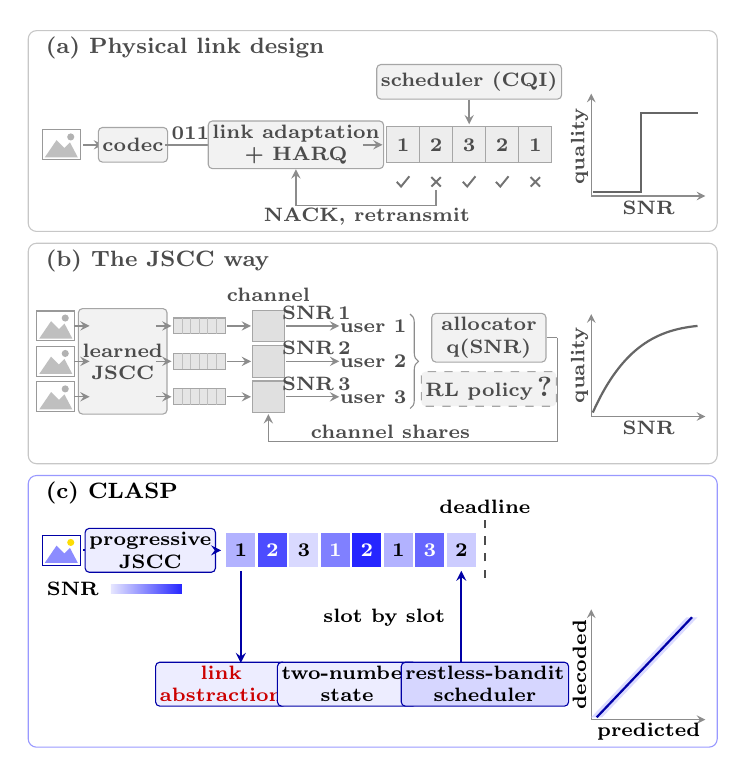
\begin{tikzpicture}[x=1cm, y=1cm, font=\footnotesize\bfseries, >=stealth,
  frame/.style={draw=black!22, rounded corners=3pt, line width=0.4pt},
  gbox/.style={draw=black!35, fill=black!5, text=black!70, rounded corners=1.5pt, align=center,
    inner sep=1.5pt, minimum height=0.44cm, font=\scriptsize\bfseries},
  cbox/.style={draw=blue!65!black, fill=blue!7, text=black, rounded corners=1.5pt, align=center,
    inner sep=1.5pt, minimum height=0.44cm, font=\scriptsize\bfseries},
  garr/.style={->, draw=black!45, line width=0.5pt},
  carr/.style={->, draw=blue!65!black, line width=0.6pt},
  gtxt/.style={text=black!70},
  small/.style={font=\scriptsize\bfseries},
  pics/gimg/.style={code={
    \draw[black!40, fill=white] (-0.24,-0.19) rectangle (0.24,0.19);
    \fill[black!25] (-0.21,-0.16) -- (-0.06,0.06) -- (0.04,-0.04) -- (0.11,0.03) -- (0.21,-0.16)
      -- cycle;
    \fill[black!30] (0.12,0.1) circle (0.045);}},
  pics/cimg/.style={code={
    \draw[blue!65!black, fill=white] (-0.24,-0.19) rectangle (0.24,0.19);
    \fill[blue!45] (-0.21,-0.16) -- (-0.06,0.06) -- (0.04,-0.04) -- (0.11,0.03) -- (0.21,-0.16)
      -- cycle;
    \fill[yellow!80!orange] (0.12,0.1) circle (0.045);}},
  pics/ok/.style={code={\draw[line width=0.7pt] (-0.08,0) -- (-0.025,-0.06) -- (0.08,0.07);}},
  pics/no/.style={code={\draw[line width=0.7pt] (-0.06,-0.06) -- (0.06,0.06)
    (-0.06,0.06) -- (0.06,-0.06);}},
]
% ---------------------------------------------------------------- (a) physical link design
\begin{scope}[yshift=0.5cm]
\draw[frame] (0,6.05) rectangle (8.75,8.6);
\node[anchor=west, gtxt] at (0.1,8.38) {(a) Physical link design};
\pic at (0.42,7.15) {gimg};
\draw[garr] (0.7,7.15) -- (0.95,7.15);
\node[gbox, minimum width=0.75cm] at (1.33,7.15) {codec};
\draw[garr] (1.74,7.15) -- (2.55,7.15);
\node[gtxt, small] at (2.14,7.3) {0110};
\node[gbox, minimum width=1.6cm] at (3.4,7.15) {link adaptation\\+ HARQ};
\draw[garr] (4.25,7.15) -- (4.5,7.15);
\foreach \i/\u in {0/1, 1/2, 2/3, 3/2, 4/1} {
  \draw[black!35, fill=black!7] (4.55+0.42*\i,6.92) rectangle (4.97+0.42*\i,7.38);
  \node[gtxt, small] at (4.76+0.42*\i,7.15) {\u};
}
\foreach \i in {0, 2, 3} \pic[black!55] at (4.76+0.42*\i,6.68) {ok};
\foreach \i in {1, 4} \pic[black!55] at (4.76+0.42*\i,6.68) {no};
\draw[garr] (5.18,6.57) |- (3.4,6.38) -- (3.4,6.84);
\node[gtxt, small] at (4.3,6.24) {NACK, retransmit};
\node[gbox, minimum width=2.1cm] (sa) at (5.6,7.95) {scheduler (CQI)};
\draw[garr] (sa.south) -- (5.6,7.41);
\draw[black!45, ->] (7.15,6.5) -- (8.6,6.5);
\draw[black!45, ->] (7.15,6.5) -- (7.15,7.8);
\draw[black!60, line width=0.8pt] (7.17,6.55) -- (7.78,6.55) -- (7.78,7.55) -- (8.5,7.55);
\node[gtxt, small] at (7.88,6.35) {SNR};
\node[gtxt, small, rotate=90] at (7.0,7.13) {quality};
\end{scope}
% ---------------------------------------------------------------- (b) the JSCC way
\draw[frame] (0,3.6) rectangle (8.75,6.4);
\node[anchor=west, gtxt] at (0.1,6.18) {(b) The JSCC way};
\node[gbox, minimum width=0.8cm, minimum height=1.34cm] (jscc) at (1.2,4.9) {learned\\JSCC};
\node[gtxt, small] at (3.05,5.75) {channel};
\foreach \k/\y in {1/5.35, 2/4.9, 3/4.45} {
  \begin{scope}[shift={(0.35,\y)}, scale=0.75] \pic {gimg}; \end{scope}
  \draw[garr] (0.58,\y) -- (0.78,\y);
  \draw[garr] (1.62,\y) -- (1.82,\y);
  \draw[black!35, fill=black!10] (1.85,\y-0.1) rectangle (2.5,\y+0.1);
  \foreach \t in {1,...,5} \draw[black!25] (1.85+0.108*\t,\y-0.1) -- (1.85+0.108*\t,\y+0.1);
  \draw[garr] (2.53,\y) -- (2.83,\y);
  \draw[black!35, fill=black!12] (2.85,\y-0.2) rectangle (3.25,\y+0.2);
  \draw[garr] (3.28,\y) -- (3.95,\y);
  \node[gtxt, small, above] at (3.66,\y-0.04) {SNR\,\k};
  \node[gtxt, small] at (4.38,\y) {user \k};
}
\draw[black!45, decorate, decoration={brace, amplitude=3pt}] (4.85,5.5) -- (4.85,4.3);
\node[gbox, minimum width=1.45cm] (al) at (5.85,5.2) {allocator\\q(SNR)};
\node[gbox, minimum width=1.45cm, dashed] (rl) at (5.85,4.55) {RL policy\,\normalsize ?};
\draw[black!45, line width=0.5pt] (al.east) -- (6.72,5.2) (rl.east) -- (6.72,4.55);
\draw[garr] (6.72,5.2) -- (6.72,3.88) -- (3.05,3.88) -- (3.05,4.23);
\node[gtxt, small] at (4.6,4.01) {channel shares};
\draw[black!45, ->] (7.15,4.2) -- (8.6,4.2);
\draw[black!45, ->] (7.15,4.2) -- (7.15,5.5);
\draw[black!60, line width=0.8pt] (7.17,4.25) .. controls (7.55,5.1) and (8.0,5.3) .. (8.5,5.35);
\node[gtxt, small] at (7.88,4.05) {SNR};
\node[gtxt, small, rotate=90] at (7.0,4.85) {quality};
% ---------------------------------------------------------------- (c) CLASP
\draw[frame, draw=blue!40] (0,0) rectangle (8.75,3.45);
\node[anchor=west] at (0.1,3.23) {(c) CLASP};
\pic at (0.42,2.5) {cimg};
\draw[carr] (0.7,2.5) -- (0.95,2.5);
\node[cbox, minimum width=1.15cm] (pj) at (1.55,2.5) {progressive\\JSCC};
\draw[carr] (pj.east) -- (2.45,2.5);
\foreach \i/\c/\u in {0/30/1, 1/70/2, 2/15/3, 3/50/1, 4/85/2, 5/30/1, 6/60/3, 7/20/2} {
  \fill[blue!\c] (2.5+0.4*\i,2.27) rectangle (2.9+0.4*\i,2.73);
  \draw[white, line width=0.8pt] (2.5+0.4*\i,2.27) rectangle (2.9+0.4*\i,2.73);
  \pgfmathsetmacro{\tc}{\c>45 ? "white" : "black"}
  \node[small, text=\tc] at (2.7+0.4*\i,2.5) {\u};
}
\draw[black!70, dashed, line width=0.6pt] (5.8,2.15) -- (5.8,2.9);
\node[small] at (5.8,3.05) {deadline};
\shade[left color=blue!10, right color=blue!85] (1.05,1.95) rectangle (1.95,2.07);
\node[small, anchor=east] at (1.02,2.01) {SNR};
\draw[carr] (2.7,2.24) -- (2.7,1.07);
\node[cbox, minimum width=1.25cm, text=red!80!black] (la) at (2.45,0.8) {link\\abstraction};
\draw[carr] (la.east) -- (3.37,0.8);
\node[cbox, minimum width=1.3cm] (st) at (4.05,0.8) {two-number\\state};
\draw[carr] (st.east) -- (4.97,0.8);
\node[cbox, minimum width=1.6cm, fill=blue!16] (rb) at (5.8,0.8) {restless-bandit\\scheduler};
\draw[carr] (5.5,1.07) -- (5.5,2.24);
\node[small, anchor=east] at (5.42,1.65) {slot by slot};
\draw[black!45, ->] (7.15,0.35) -- (8.6,0.35);
\draw[black!45, ->] (7.15,0.35) -- (7.15,1.75);
\fill[blue!14] (7.15,0.38) -- (7.29,0.38) -- (8.5,1.65) -- (8.36,1.65) -- cycle;
\draw[blue!65!black, line width=0.8pt] (7.22,0.38) -- (8.43,1.65);
\node[small] at (7.88,0.2) {predicted};
\node[small, rotate=90] at (7.0,1.05) {decoded};
\end{tikzpicture}

\caption{Approaches to serving images to many users over a fading downlink. (a) Physical link
design transmits the bits of a separate codec at a rate set from a channel report. Every block
either decodes or fails, and HARQ resends a failed block in a later slot. (b) JSCC design transmits
a learned code, and its scheduler splits the channel among users according to a quality predicted
at one SNR or a policy learned by reinforcement learning. (c) CLASP schedules a progressive code
trained under slot-varying SNR, whose link abstraction values every slot. This restless-bandit
scheduler serves every user slot by slot up to the deadline.}
\label{fig:overview}
\end{figure}

Although JSCC design avoids the cliff effect of physical link design, it leaves three challenges
unresolved:
\begin{itemize}
\item \emph{Absence of a link abstraction}: The quality models of JSCC design, whether fitted curves
or learned predictors \cite{Yan22,Zhang23,Hou26}, take a single SNR as input. Each model maps this
SNR to the predicted quality of a whole image, as if every symbol of the image met the same channel.
Physical link design provides rules for the error rate of a digital block, namely the exponential
and mutual-information effective SNR mappings (EESM and MIESM) \cite{Ericsson03,EMD09}. To our
knowledge, no comparable rule has been reported for how the SNRs of the slots that carry one image
combine into the quality of a nonlinear code.
\item \emph{Absence of tractable and certifiable scheduling}: Choosing the users of every slot up to 
the deadline, without knowledge of future slots, is a stochastic dynamic program whose state grows
exponentially with the number of users. The quality-based allocations are myopic, since they ignore
the slots that remain in the frame \cite{Yan22,Xia24,Hou26}. Learned policies
\cite{Wang22,Zhang23t,McDowell26} require many training interactions and offer no certificate of
their distance from the optimum.
\item \emph{Imperfect information}: The scheduler makes decisions based on predictions of both the
quality and the channel, both of which are imperfect. Per-image rate selection \cite{Zhang23}
treats its predicted quality as exact, so a user predicted just above a quality target may decode
just below it. The learned restless-bandit scheduler likewise assumes exact channel knowledge
\cite{McDowell26}. Moreover, the advantage that motivates these designs was measured against an
idealized digital link with exact channel knowledge and capacity-achieving codes
\cite{Bourtsoulatze19,Kurka20}. Whether this advantage persists under the reports of a real base
station remains open.
\end{itemize}

The first challenge underlies the other two, since a scheduler needs a link abstraction both to plan
over the remaining slots with a certificate and to account for prediction errors. We therefore ask
whether the decoded quality of a learned code can be predicted from its slot SNRs at all, and how
the code should be trained to make this possible. To answer these questions, we trained the same
progressive architecture in two ways, under slot-varying SNR and at one constant SNR per image. We
then compared candidate rules on both codes and evaluated the most accurate rule within a scheduler
(Sections~\ref{sec:method-abstraction}, \ref{sec:eval-abstraction} and~\ref{sec:eval-ablation}).
Three findings emerged. First, the code trained under slot-varying SNR has an additive link
abstraction, a property that linear analog codes have by construction \cite{Jakubczak11}. A source
term plus a weighted sum of per-slot minimum mean-square-error (MMSE) terms predicts its decoded
quality more accurately than EESM and MIESM. Second, the training condition determines whether the
abstraction holds. For the code trained at one constant SNR per image, none of the candidate rules
predicts the decoded quality with comparable accuracy. Third, the abstraction remains accurate on
the slots that a scheduler selects. It can be calibrated for each image from a small number of
decodes, but the calibrated predictions retain a residual error. A scheduler that ignores this error
leaves more users below a quality target than one that models it. These findings indicate that a
scheduler can rely on the link abstraction of a code trained under slot-varying SNR, provided that
it accounts for this error.

We therefore propose CLASP (Cal\-i\-bra\-tion-aware Link-Ab\-strac\-tion-based Scheduling of
Progressive codes), a scheduler for learned progressive codes over a multi-user fading downlink.
Unlike the restless-bandit schedulers for layered video \cite{Hosseini19} and learned semantic codes
\cite{McDowell26}, CLASP values each slot through the link abstraction instead of a decode-or-fail
outcome or reinforcement learning. The abstraction reduces the state of each user to two numbers,
namely the length of the prefix received so far and its accumulated weighted noise. Deadline
scheduling over these states is thus a finite-horizon restless bandit problem \cite{Whittle88}, and
its Lagrangian relaxation decomposes into one small dynamic program per user. Solving these programs
exactly yields the Lagrangian index by which CLASP selects the users of each slot, together with an
upper bound on the achievable performance \cite{Brown20,Hao22}. Each program rewards the probability
of reaching the quality target under the measured errors of the abstraction and of the channel
reports. Experiments show that CLASP outperforms proportional fair scheduling, per-image rate
selection and a digital chain with link adaptation and HARQ.

The main contributions of this paper are as follows:
\begin{itemize}
\item We show that a progressive code obeys an additive MMSE link abstraction when it is trained
under slot-varying SNR, but not when it is trained at one constant SNR per image. The mean absolute
error of this abstraction is 0.055--0.083~dB on two test sets, well below the 0.16--0.19~dB of EESM
and the 0.29--0.34~dB of MIESM.
\item We propose CLASP as a restless-bandit scheduler with exact per-user dynamic programs, whose
reward accounts for the errors of both the quality predictions and the channel reports.
\item When every scheduled delivery is decoded by the codec, CLASP gains 0.5--0.6~dB of mean PSNR
over proportional fair scheduling. It also brings an extra 8--15\% of the users to 30~dB over 
per-image rate selection. Simulated against a digital chain with CQI-table link adaptation and 
HARQ, it gains 1.2--1.6~dB of mean PSNR under 2~dB CQI errors or reports aged to correlation 0.8. 
Its simulated gap to the upper bound falls to 0.005~dB per user at 128 users. Training the code on 
the channel that CLASP creates raises the decoded mean PSNR by a further 0.21~dB.
\end{itemize}

The rest of the paper is organized as follows. Section~\ref{sec:related} reviews related work, and
Section~\ref{sec:system} states the system model and the problem. Section~\ref{sec:method} presents
the training of the progressive code, its MMSE link abstraction, CLASP, and the training of the code
on the channel CLASP creates. Section~\ref{sec:eval} evaluates the abstraction, and CLASP against
PF, per-image rate selection, the Lagrangian bound and the digital chain. Section~\ref{sec:conclusion}
concludes and states the limitations.


\section{Related Work}
\label{sec:related}

\subsection{Physical Link Design for Multi-User Media Delivery}
\label{sec:related-link}

\subsection{The JSCC Way}
\label{sec:related-jscc}

\subsection{Restless Bandits and Lagrangian Index Policies}
\label{sec:related-rmab}

\section{Preliminaries: System Model and Problem Statement}
\label{sec:system}

\section{Method}
\label{sec:method}

\subsection{Training the Progressive Code for Slot-Varying SNR}
\label{sec:method-training}

\subsection{The MMSE Link Abstraction}
\label{sec:method-abstraction}

\subsection{CLASP: Deadline Scheduling as a Finite-Horizon Restless Bandit}
\label{sec:method-clasp}

\subsection{Imperfect Information: The Calibration-Aware Reward and Aged Reports}
\label{sec:method-csi}

\subsection{Training the Code on the Channel CLASP Creates}
\label{sec:method-codesign}

\section{Experiments}
\label{sec:eval}

\subsection{Link Abstraction Accuracy}
\label{sec:eval-abstraction}

\subsection{Mean PSNR: Near the Bound, and over PF}
\label{sec:eval-mean}

\subsection{Quality Target and Latency}
\label{sec:eval-target}

\subsection{Imperfect CSI and the Digital Baseline}
\label{sec:eval-csi}

\subsection{Training the Code on CLASP's Channel}
\label{sec:eval-codesign}

\subsection{Ablations and System Choice}
\label{sec:eval-ablation}

\section{Conclusion}
\label{sec:conclusion}

\IEEEtriggercmd{\balance}
\IEEEtriggeratref{14}

\bibliographystyle{IEEEtran}
\bibliography{references}

\end{document}
